\documentclass[11pt,a4paper]{article}
 
\usepackage[T1]{fontenc}
\usepackage[portuguese]{babel}
\usepackage{authblk}
\usepackage{enumitem}
\usepackage{graphicx}
\usepackage[hmargin=2cm,vmargin=3.5cm,bmargin=2cm]{geometry}


\newcommand{\select}{\mbox{\Large$\sigma$}}

\pagenumbering{arabic}

\title{\textbf{Projecto de Base de Dados}}
 
\author{Bruno Cardoso, Lidia Freitas e Rodrigo Bernardo} 

\affil{Instituto Superior T\'{e}cnico}
 
\date{Parte 1}
 
\begin{document}

\maketitle

\newpage


\tableofcontents %Índice de conteúdos
\newpage
\setcounter{page}{1}
\section{O Modelo}
\subsection{Modelo Entidade-Associa\c{c}\~ao}

%\advance\leftskip-5.0cm
\centerline{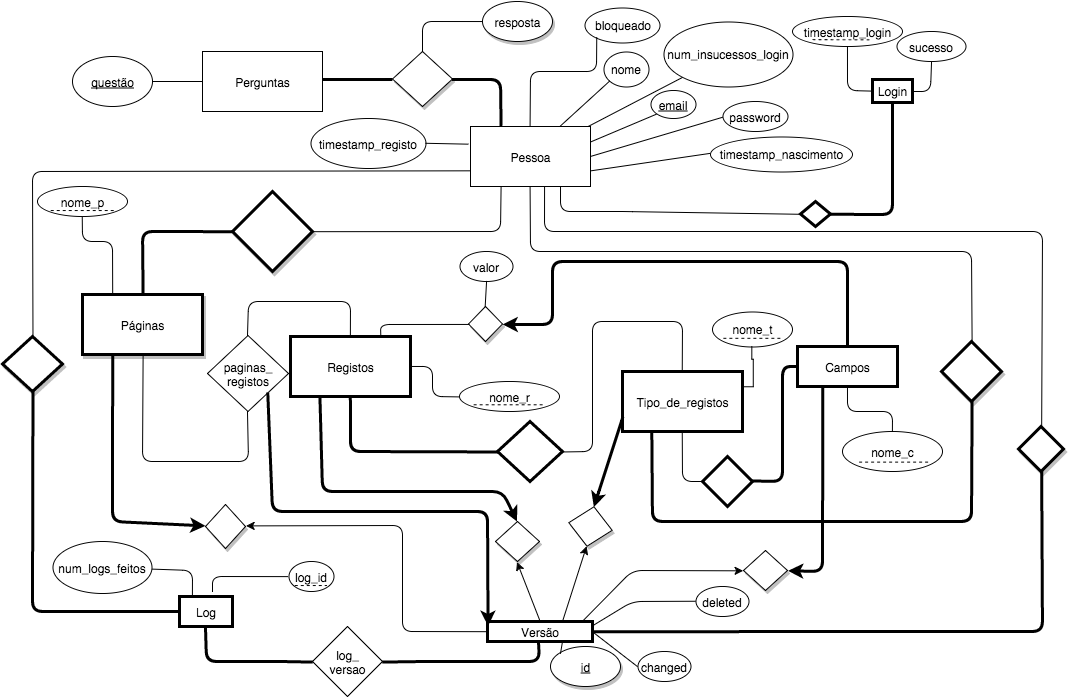
\includegraphics[width=1.0\textwidth]{modelo-ea.png}}
%\advance\leftskip+2.5cm


ADICIONAR CHAVE CANDIDATA A PESSOA.(Alternativa de entrar na conta)
\newpage
\subsection{Restri\c{c}\~oes de Integridade do Modelo Entidade-Associa\c{c}\~ao}

\paragraph{}

O Modelo Entidade-Associa\c{c}\~{a}o, apenas com o diagrama, n\~{a}o exige que n\~{a}o ocorram situa\c{c}\~{o}es fora do dom\'{\i}nio do problema.




\section{Modelo Relacional}
\subsection{O Modelo}

\begin{description}[noitemsep]
	\item Pergunta(\underline{quest\~ao, email}, resposta)
	\item email: FK(Pessoa)
	\item notnull(resposta)
\end{description}

\begin{description}[noitemsep]
	\item Pessoa(\underline{email}, bloqueado, nome, num\_insucessos\_login, password, timestamp\_nascimento, timestamp\_registo, num\_undos)
	\item notnull(email)
	\item notnull(bloqueado)
	\item notnull(nome)
	\item notnull(num\_insucessos\_login)
	\item notnull(password)
	\item notnull(timestamp\_nascimento)
	\item notnull(timestamp\_registo)
	\item notnull(num\_undos)
\end{description}

\begin{description}[noitemsep]
	\item Login(\underline{timestamp\_login, email}, sucesso)
	\item email: FK(Pessoa)
	\item notnull(sucesso)
\end{description}

\begin{description}[noitemsep]
	\item P\'{a}ginas(\underline{nome\_p, email}, id)
	\item email: FK(Pessoa)
	\item id: FK(Pessoa)
	\item notnull(id)
\end{description}

\begin{description}[noitemsep]
	\item P\'{a}ginas\_registos(\underline{nome\_p, email, nome\_r, nome\_t},id )
	\item nome\_p, email: FK(P\'{a}ginas)
	\item nome\_r, nome\_t, email: FK(Registos)
	\item id: FK(Vers\~{a}o)
	\item notnull(id)
\end{description}

\begin{description}[noitemsep]
	\item Registos(\underline{nome\_r, nome\_t, email}, id)
	\item nome\_t, email: FK(tipos\_de\_registos)
	\item id: FK(Vers\~{a}o)
	\item notnull(id)
\end{description}

\begin{description}[noitemsep]
	\item Tipos\_de\_registos(\underline{nome\_t, email}, id)
	\item email: FK(Pessoa)
	\item notnull(id)
	\item id: FK(Vers\~{a}o)
\end{description}
\newpage

\begin{description}[noitemsep]
	\item Campos(\underline{nome\_c, nome\_t, email}, id)
	\item nome\_t, email: FK(Tipo\_de\_registos)
	\item id: FK(Vers\~{a}o)
	\item notnull(id)
\end{description}

\begin{description}[noitemsep]
	\item Registo\_Campos(\underline{nome\_r, nome\_t, nome\_c, email}, id)
	\item nome\_r, nome\_t, email: FK(Registos)
	\item nome\_c, nome\_t, email: FK(Campos)
	\item id: FK(Vers\~{a}o)
	\item notnull(id)
\end{description}


\begin{description}[noitemsep]
	\item Vers\~{a}o(\underline{id}, changed, deleted)
	\item notnull(changed)
	\item notnull(deleted)
\end{description}

\begin{description}[noitemsep]
	\item Log(\underline{log\_id, email})
	\item email: FK(Pessoa)
\end{description}

\begin{description}[noitemsep]
	\item Log\_vers\~{a}o(\underline{log\_id, email, id})
	\item log\_id, email: FK(Log)
	\item id: FK(Vers\~{a}o)
\end{description}

\subsection{Restri\c{c}\~oes de Integridade do Modelo Relacional}
\section{\'{A}lgebra Relacional}
\subsection{Pergunta 1}

$\Pi_{nome\_t}(\sigma_{email = 'Manel@Notebook.pt'}(Tipo\_de\_registos))$

\subsection{Pergunta 2}

Pessoa $\bowtie \Pi_{email}$ ( $\select_{sucesso=falso} (login)$ )

\subsection{Pergunta 3}








\section{Linguagem SQL}
\subsection{Pergunta 1}
SELECT DISTINCT nome\_t
\\FROM Tipo\_de\_registos
\\WHERE email="Manel@notebook.pt";

\subsection{Pergunta 2}
SELECT DISTINCT Pessoa.* 
\\FROM Pessoa, Login 
\\WHERE Pessoa.email = Login.email AND sucesso = false;

\subsection{Pergunta 3}
SELECT timestamp\_nascimento
\\FROM Pessoa, Paginas, Registos 
\\WHERE Pessoa.email = Registos.email 
\\AND Pessoa.email = Paginas.email 
\\AND nome\_p = "facebook" 
\\AND nome\_r = "facebook";








\end{document}